\documentclass[border=6pt]{standalone}
\usepackage{amsmath,amssymb}
\usepackage{tikz}
\usetikzlibrary{arrows.meta,calc,decorations.pathreplacing,patterns,shapes.geometric,positioning,shadings,plotmarks}

\begin{document}
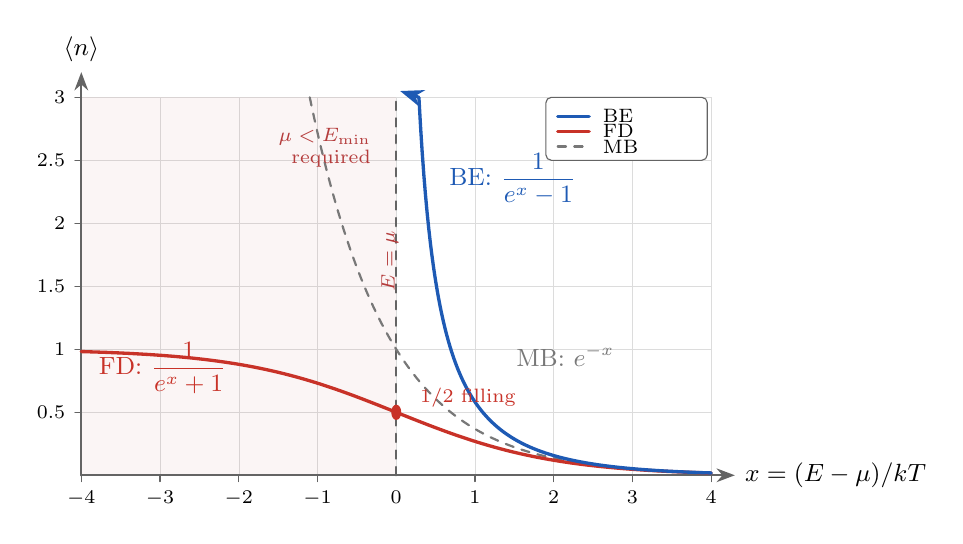
\begin{tikzpicture}[>=Stealth, line cap=round, line join=round]

% Colors
\definecolor{BEblue}{RGB}{30,90,180}
\definecolor{FDred}{RGB}{200,50,40}
\definecolor{MBgray}{RGB}{120,120,120}
\definecolor{axisgray}{RGB}{100,100,100}
\definecolor{gridgray}{RGB}{220,220,220}
\definecolor{forbidpink}{RGB}{180,60,60}

% Axes scale: x from -4 to 4 (1 unit = 1 cm), y from 0 to 3 (1 unit = 1.6 cm)
\def\xmin{-4}
\def\xmax{4}
\def\ymin{0}
\def\ymax{3}
\pgfmathsetmacro{\xscale}{1.0}
\pgfmathsetmacro{\yscale}{1.6}

% Coordinate system
\begin{scope}[xscale=\xscale, yscale=\yscale]

% Light grid
\foreach \xg in {-4,-3,-2,-1,0,1,2,3,4}{
  \draw[gridgray, very thin] (\xg,\ymin) -- (\xg,\ymax);
}
\foreach \yg in {0.5,1,1.5,2,2.5,3}{
  \draw[gridgray, very thin] (\xmin,\yg) -- (\xmax,\yg);
}

% Forbidden region for BE: x < 0 shaded subtle
\fill[forbidpink, opacity=0.05] (\xmin,\ymin) rectangle (0,\ymax);

% Vertical line at x=0 (E = mu)
\draw[axisgray, dashed, thick] (0,\ymin) -- (0,\ymax);
\node[forbidpink, font=\scriptsize, anchor=south, rotate=90] at (0.15,1.7) {$E=\mu$};

% Axes
\draw[axisgray, thick, ->] (\xmin,0) -- (\xmax+0.3,0) node[right, black, font=\small] {$x=(E-\mu)/kT$};
\draw[axisgray, thick, ->] (\xmin,0) -- (\xmin,\ymax+0.2) node[above, black, font=\small] {$\langle n\rangle$};

% X ticks
\foreach \xt in {-4,-3,-2,-1,1,2,3,4}{
  \draw[axisgray] (\xt,0) -- (\xt,-0.05);
  \node[below, font=\scriptsize, black] at (\xt,-0.05) {$\xt$};
}
\node[below, font=\scriptsize, black] at (0,-0.05) {$0$};

% Y ticks
\foreach \yt/\ylab in {0.5/0.5, 1/1, 1.5/1.5, 2/2, 2.5/2.5, 3/3}{
  \draw[axisgray] (\xmin,\yt) -- (\xmin-0.08,\yt);
  \node[left, font=\scriptsize, black] at (\xmin-0.08,\yt) {\ylab};
}

% MB curve: e^{-x}, plot from x=-1.1 to x=4 (clip at y=3)
\draw[MBgray, thick, dashed, samples=140, domain=-1.0986:4]
  plot (\x, {min(exp(-\x),3)});

% FD curve: 1/(e^x+1), plot from x=-4 to x=4
\draw[FDred, very thick, samples=160, domain=-4:4]
  plot (\x, {1/(exp(\x)+1)});

% BE curve: 1/(e^x - 1), plot from x=0.36 to x=4 (where 1/(e^x-1) is below 3 at x=ln(4/3)=0.2877; pick safe start)
% At x=0.3466, 1/(e^x-1)=2.42; at x=0.288, ~3. Start near 0.288.
\draw[BEblue, very thick, samples=180, domain=0.288:4]
  plot (\x, {1/(exp(\x)-1)});

% BE diverging arrow tip
\draw[BEblue, very thick, ->] (0.288,3) -- (0.05,3.05);

% FD point at (0,1/2)
\filldraw[FDred] (0,0.5) circle (1.6pt);
\node[FDred, font=\scriptsize, anchor=west] at (0.18,0.62) {$1/2$ filling};

% Labels for curves
\node[BEblue, font=\small, anchor=west] at (0.55, 2.35) {BE: $\dfrac{1}{e^x-1}$};
\node[FDred, font=\small, anchor=west] at (-3.9, 0.85) {FD: $\dfrac{1}{e^x+1}$};
\node[MBgray, font=\small, anchor=west] at (1.4, 0.95) {MB: $e^{-x}$};

% BE forbidden label
\node[forbidpink, font=\scriptsize, anchor=east, align=right] at (-0.2, 2.6) {$\mu<E_{\min}$\\required};

% Legend (top right)
\begin{scope}[shift={(2.0,2.55)}]
  \draw[fill=white, draw=axisgray, thin, rounded corners=2pt] (-0.1,-0.05) rectangle (1.95,0.45);
  \draw[BEblue, very thick] (0.05,0.30) -- (0.45,0.30);
  \node[font=\scriptsize, anchor=west, black] at (0.5,0.30) {BE};
  \draw[FDred, very thick] (0.05,0.18) -- (0.45,0.18);
  \node[font=\scriptsize, anchor=west, black] at (0.5,0.18) {FD};
  \draw[MBgray, thick, dashed] (0.05,0.06) -- (0.45,0.06);
  \node[font=\scriptsize, anchor=west, black] at (0.5,0.06) {MB};
\end{scope}

\end{scope}

\end{tikzpicture}
\end{document}
